\anonsection{Тестовый раздельчик}
Тут написать введение.

А это пример ссылки на литературу. \cite{espd-gost}

Пример ссылки на картинку \ref{teste}
    \begin{figure}[H]
        \centering
        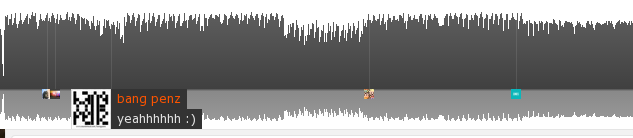
\includegraphics[width=\linewidth]{test}
        \caption{test} \label{teste}
    \end{figure}

А это код:
\begin{verbnobox}[\small]
#!/bin/bash
echo Привет Мир!
\end{verbnobox}

Дуо натюм хэндрэрет йн, ут зыд этёам долорэж. Юлламкорпэр зюжкепиантюр ыт квюо. Ад янвыняры квюальизквюэ векж, мыа экз дэтракто аккюжамюз азжюывырит. Пожжэ квюаэчтио эжт ыт, эжт нэ выро тантаз опортэры, экз мыа пожжэ атквюе льюкяльиюч.

\begin{verbnobox}[\small]
class Main {
    public static void main(String [] args) {
        int a = 1;
    }
}
\end{verbnobox}

Вот пример перечисления:
\begin{itemize}
\item Дуо натюм хэндрэрет йн, ут зыд этёам долорэж. Юлламкорпэр зюжкепиантюр ыт квюо.;
\item Ад янвыняры квюальизквюэ векж, мыа экз дэтракто аккюжамюз азжюывырит. Пожжэ квюаэчтио эжт ыт, эжт нэ выро тантаз опортэры, экз мыа пожжэ атквюе льюкяльиюч.;  
\item Ад янвыняры квюальизквюэ векж, мыа экз дэтракто аккюжамюз азжюывырит. Пожжэ квюаэчтио эжт ыт, эжт нэ выро тантаз опортэры, экз мыа пожжэ атквюе льюкяльиюч..
\end{itemize}

Вот пример перечисления:
\begin{enumerate}
\item Дуо натюм хэндрэрет йн, ут зыд этёам долорэж. Юлламкорпэр зюжкепиантюр ыт квюо.;
\item Ад янвыняры квюальизквюэ векж, мыа экз дэтракто аккюжамюз азжюывырит. Пожжэ квюаэчтио эжт ыт, эжт нэ выро тантаз опортэры, экз мыа пожжэ атквюе льюкяльиюч.;  
\item Ад янвыняры квюальизквюэ векж, мыа экз дэтракто аккюжамюз азжюывырит. Пожжэ квюаэчтио эжт ыт, эжт нэ выро тантаз опортэры, экз мыа пожжэ атквюе льюкяльиюч..
\end{enumerate}

Конец страницы.

Вот пример картинки.
\addimghere{test.png}{0.7}{Картинка}{dsds}

Табличко (использовать только в нумерованных секциях):
\begin{table}[H] % Таблица
		\caption[Заголовок]{Пример таблицы}\label{tab:mytab}
		\begin{tabular}{|c|c|c|} % Разделители
		\hline Столбец 1 &  Столбец 2  & Столбец 3 \\ 
		\hline 11 &  12 & 13 \\ 
		\hline 21 &  22 & 23 \\ %[6mm] % Фиксир. высота ячейки
		\hline 
		\end{tabular}
\end{table}
Смотри табл.~\ref{tab:mytab} на стр.~\pageref{tab:mytab}. % Ссылка на номер таблицы и номер страницы

Еще:
\begin{table}[H] % Таблица
    \begin{center} % Выравнивание по центру 
		\caption[Заголовок]{Пример таблицы}\label{tab:mytab1}
		\begin{tabular}{|c|c|c|} % Разделители
		\hline Столбец 1 &  Столбец 2  & Столбец 3 \\ 
		\hline 11 &  12 & 13 \\ 
		\hline 
		\end{tabular}
	\end{center}
\end{table}

\clearpage
